\section{Visualising data}
\paragraph{}
The data we are going to use is present in a file of type \lstinline{Rdata} and it consists of two parts: data for \emph{training} and data for \emph{testing}.
Each dataset has a number of $75$ instances (an instance being described by $2$ \emph{features}) which are divided (not equally) amongst $3$ \emph{classes}.

\paragraph{}
Having a \emph{true class} assigned to each instance, we can treat this problem as a \emph{supervised classification} problem.
Moreover, we also have information about true \emph{means} and \emph{standard deviations}, so we can use these to make comparisons between our algorithms and the truth.

\paragraph{}
Let's take a look at how the data looks:

\begin{figure}[H]
    \centering
    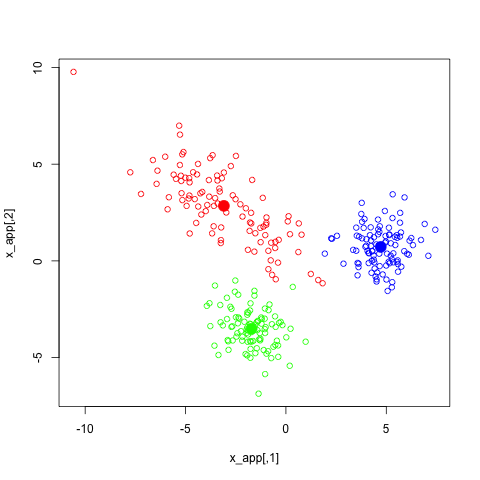
\includegraphics[width=\textwidth/2 - 10pt]{train_data.png}
    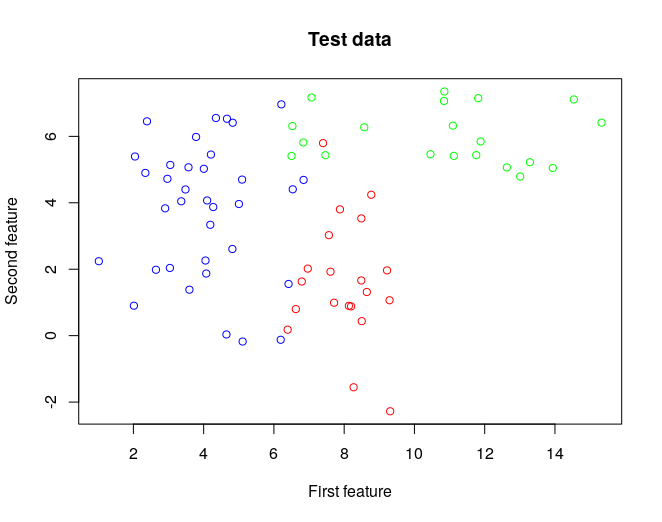
\includegraphics[width=\textwidth/2 - 10pt]{test_data.png}
    \caption{Plotted data. Train on left, test on right}
    \label{data}
\end{figure}

\begin{lstlisting}[language=R, caption=Loading and visualising data]
data <- load(file='simul-2017.Rdata')
class_colors = c('red', 'green', 'blue')
couleur <- rep('red', n_app)
for (class_no in 1:3)
  couleur[classe_app == class_no] = class_colors[class_no]
# plot data
plot (x_app, col=couleur, main='Training data', xlab='1st feature', ylab='2nd feature')
for (class_no in 1:3)
  couleur[classe_test == class_no] = class_colors[class_no]
plot (x_test, col=couleur, main='Test data', xlab='1st feature', ylab='2nd feature')
\end{lstlisting}

\clearpage

\paragraph{}
We can notice more blue dots, which would mean instances are not equally distributed amongst classes.
Calculating the class a priori probabilities, that is indeed true:
\begin{lstlisting}[language=R, caption=A priori class probabilities]
# P(w) = probability of an instance to be in the class "w"
class_probs_app <- 1:3
class_probs_test <- 1:3
for (class_no in 1:3){
    class_probs_app[class_no] = sum(class_no == classe_app) / length(classe_app)
    class_probs_test[class_no] = sum(class_no == classe_test) / length(classe_test)
}
class_probs_app
class_probs_test
\end{lstlisting}

\paragraph{}
The script above gives us the values $P(red) = 0.28$, $P(green) = 0.3466667$ and $P(blue) = 0.3733333$ for the training dataset and $P(red) = 0.2666667$, $P(green) = 0.2666667$ and $P(blue) = 0.4666667$, for the test dataset.
The values corresepond to red, green and blue classes, in this order.


\section{Estimating means and covariance}

\subsection{Calculating means}

\paragraph{}
A first small step to analysing the data would be to look at the ``centroids'' for each class, that is calculating the means for each class.

\begin{lstlisting}[language=R, caption=Calculating means]
# calculate means
means <- array(dim = c(3, 2))
for (class_no in 1:3){
    means[class_no, 1] <- mean (x_app[classe_app == class_no, 1])
    means[class_no, 2] <- mean (x_app[classe_app == class_no, 2])
}
# plot the means for train data
for (class_no in 1:3)
    couleur[classe_app == class_no] = class_colors[class_no]
plot (x_app, col=couleur, main='Means for train data', xlab='First feature', ylab='Second feature')
points (means, col=class_colors, p=8, cex=4)
\end{lstlisting}

\begin{figure}[H]
    \centering
    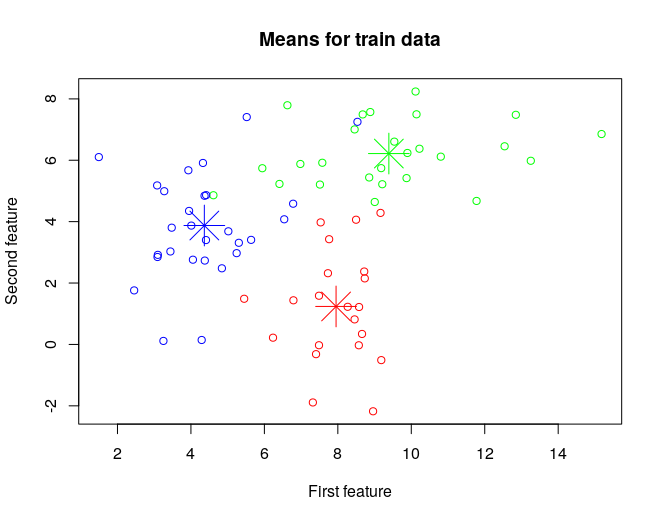
\includegraphics[scale=0.5]{means_train.png}
    \caption{Visualising means with instances}
    \label{}
\end{figure}

\clearpage

\begin{center}
    \begin{tabular}{ cc }   % top level tables, with 2 rows
        True results & My results \\  
        % bottom left of the top level table: table 1 
        \begin{tabular}{ |c|c|c|c| } 
        \hline
        & Red & Green & Blue\\
        X1 & 8 & 10 & 4 \\
        X2 & 1 & 6 & 4 \\
        \hline
        \end{tabular} &  % starting bottom right of the top level table
        % table 2
        \begin{tabular}{ |c|c|c|c| } 
        \hline
        & Red & Green & Blue\\
        X1 & 7.951986 & 9.389311 & 4.365176 \\
        X2 & 1.237545 & 6.218550 & 3.874318 \\
        \hline
        \end{tabular} \\
    \end{tabular}
\end{center}

\paragraph{}
The values\footnote{The means were calculating only on the training dataset, not on all of the instances} aren't so distant from the ground truth, so we can consider them insightful.

\subsection{Covariance matrix}

\paragraph{}
Up next, we will calculate the covariance matrix.
According to \cite{covariance}, covariance is a measure of how one feature changes in relation to another.
Depending on the algorithm we're using, if two features are \emph{strongly} correlated, it might be better to let one go, in order to reduce the \emph{dimensionality} of the problem and make algorithms faster.
But, for example, algorithms like Naive Bayes might actually benefit from correlated features.
In our case, we only have $2$ features and $75$ instances, so the dimensionality of the problem doesn't really pose a problem for us.

\begin{lstlisting}[language=R, caption=Calculating covariance]
sigma <- c()
for (class_no in 1:3){
    # number of instances = n_app = dim(x_app)[1]
    # number of features = dim(x_app)[2]
    sigma[[class_no]] <- matrix(1, dim(x_app)[2], dim(x_app)[2])
    for (i in 1:dim(x_app)[2])
    for (j in 1:dim(x_app)[2])
        sigma[[class_no]][i, j] <- cov(as.vector(x_app[classe_app == class_no, i]), as.vector (x_app[classe_app == class_no, j]))
}
\end{lstlisting}

\paragraph{}
Below, we can find the script's result. For each class, we have calculated the \emph{covariance matrix}.
On the diagonal of each ${\Sigma}_i$ matrix, we have the \emph{variance} of each feature, and any other element ${\Sigma}_(j, k), j \neq k$, represents the correlation between the features $j$, $k$.
Of course, these matrixes are symmetric.

\[ 
    {\Sigma}_1 = 
    \left(\begin{array}{cc}
    0.95337723 & 0.09544548 \\
    0.09544548 & 3.26152120 \\
    \end{array} \right)
    , 
    {\Sigma}_2 = 
    \left( \begin{array}{cc}
    5.8526867 & 0.6107413 \\
    0.6107413 & 1.0474417 \\
    \end{array} \right)
    ,
\]
\[
    {\Sigma}_3 = 
    (\begin{array}{cc}
    2.0251769 & 0.7214545 \\
    0.7214545 & 3.0809579 \\
    \end{array})
\]

\[ 
    {\sigma}_1 = 
    \left(\begin{array}{cc}
    1 & 2 \\
    \end{array} \right)
    , 
    {\sigma}_2 = 
    \left( \begin{array}{cc}
    3 & 1 \\
    \end{array} \right)
    {\sigma}_3 = 
    \left( \begin{array}{cc}
    1.5 & 2 \\
    \end{array} \right)
\]

\paragraph{}
By ${\Sigma}_i$ we denoted the covariance matrix, and by ${\sigma}_i$ the ground truth regarding standard deviation.

\subsection{Analysing diagonal values}
\paragraph{}
Looking at the values on the diagonal and comparing them (! by not forgetting to raise the standard deviation, that is values from ${\sigma}_i$, to the power of 2, so we get variance), to the true values, we can see that overall they are pretty close.
The only exception is the variance for the first feature, for the second class; those aren't very similar ($\approx 5.8$ vs. $3^2$).
To cite \cite{variance}, variance ``measures how far a set of (random) numbers are spread out from their average value''.
That being said, it gives us a sense of dispersity in our data.

\paragraph{}
Now let's apply the above observations to our data\footnote{The covariance matrixes were calculated on the training data, so the observations we made are for that dataset}.
Before this, please note that in our plots above \ref{data}, the first feature $X_1$ was projected on the abscissa and the second feature $X_2$ on the ordinate.
Looking at the red class and variance for the first atribute, we could that, for the first feature, the variance is not that high.
That would mean that the red-class instances, projected on the x-axis, would be "gathered" around.
If we look at the image, that is, indeed, true! 

\paragraph{}
Thinking the other way around, if we look at the figure\ref{data} at $X_1$ for the green class, we can notice that the projections on the x-axis for the instances are quite dispersed.
That would mean that the variance for that case is higher.
And that is, once again, true (variance of $\approx 5.8$ in our results), proof that our algorithm makes the cut.

\subsection{Analysing correlation between features}
\paragraph{}
Let us now note ${\Sigma}_i(j, k) = x$, a correlation between two features.
Further analysing each possible value for $x$, we must take into account the following observations: if $x$ is positive, then if the feature $j$ increases, then so does the value for $k$.
If $x$ is negative, then if feature $j$ increases, then the value for $k$ decreases.
If $x$ is 0, then the features are not correlated.
We say that two features $j$ and $k$ are strongly correlated when the $x$ is large.